\section{Directive-Based Programming Models}\label{sec:directive-based-programming-models}


\par
The most common directive-based models for GPU parallel programming are OpenACC and OpenMP offloading approaches.
The parallelization is done by introducing directives in places which are targeted for parallelization.
\begin{itemize}
    \item OpenACC is known to be more~\textbf{descriptive}, which means the programmer uses directives to tell the compiler how/where to parallelize the code and to move the data.
    \item OpenMP offloading approach, on the other hand, is known to be more~\textbf{prescriptive}, where the programmer uses directives to tell the compiler more explicitly how/where to parallelize the code, instead of letting the compiler decides.
\end{itemize}


\par
In OpenMP/OpenACC, the compiler directives are specified by using~\textbf{\textcolor{red}{\#pragma}} in C/C++ or as special comments identified by unique sentinels in Fortran.
Compilers can ignore the directives if the support for OpenMP/OpenACC is not enabled.
The compiler directives are used for various purposes: for thread creation, workload distribution (work sharing), data-environment management, serializing sections of code or for synchronization of work among the threads.


% -------------------------------------------------------------------- %


\subsection{Execution model}


\par
OpenMP and OpenACC use the fork-join model (Fig.~\ref{fig:fork_join}) of parallel execution.
The program begins as a single thread of execution, the master thread, which executes sequentially until the first parallel region construct is encountered.
When a parallel region is encountered, the master thread creates a group of threads, becomes the master of this group of threads, and is assigned the thread index 0 within the group (the green blocks in parallel regions in Fig.~\ref{fig:fork_join}).
There is an implicit barrier at the end of the parallel regions.
When the group of threads complete the statements in the parallel region construct, they synchronize and terminate, leaving only the master thread.
It is noted that the number of parallel regions and the threads that comprise them are arbitrary.


\begin{figure}[!htbp]
\centering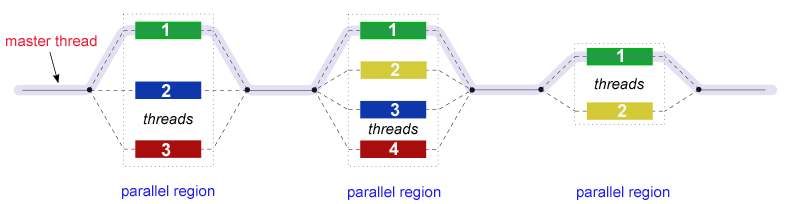
\includegraphics[width=0.8\textwidth]{fig_hardware/fork_join_model.png}
\caption{The fork-join model for parallel execution.}\label{fig:fork_join}
\end{figure}


% -------------------------------------------------------------------- %


\subsection{Offloading directives}


\subsubsection{OpenACC}


\par
In OpenACC, one of the most commonly used directives is~\textbf{\textcolor{red}{kernels}}, which defines a region to be transferred into a series of kernels to be executed in sequence on a GPU.
Work sharing is defined automatically for the separate kernels, but tuning prospects is limited.
Herein we provide code examples for OpenACC kernels in C++ and Fortran in List~\ref{lst:07_openacc_kernel_cpp} and List~\ref{lst:07_openacc_kernel_fortran}, respectively.


\lstinputlisting[language=c++, caption={Code example for OpenACC~\textbf{\textcolor{red}{kernels}} in C++. The 17$^{th}$ line indicates the starting point of OpenACC~\textbf{\textcolor{red}{kernels}}.}, label={lst:07_openacc_kernel_cpp}, xleftmargin=0.05\textwidth, xrightmargin=0.05\textwidth]{code_examples/07_openacc_kernel_cpp.cpp}


\lstinputlisting[language=fortran, caption={Code example for OpenACC~\textbf{\textcolor{red}{kernels}} in Fortran. The 14$^{th}$ and 18$^{th}$ lines indicate the starting and ending of the OpenACC~\textbf{\textcolor{red}{kernels}}.}, label={lst:07_openacc_kernel_fortran}, xleftmargin=0.05\textwidth, xrightmargin=0.05\textwidth]{code_examples/07_openacc_kernel_fortran.f}


\par
The other approach of OpenACC to define parallel regions is to use~\textbf{\textcolor{red}{parallel}} directive.
Contrary to the~\textbf{\textcolor{red}{kernels}} directive, the~\textbf{\textcolor{red}{parallel}} directive is more explicit and requires more analysis by the programmer.
Work sharing has to be defined manually using the~\textbf{\textcolor{red}{loop}} directive, and refined tuning is possible to achieve.
The code examples shown in List~\ref{lst:07_openacc_kernel_cpp} and List~\ref{lst:07_openacc_kernel_fortran} can be rewritten using the~\textbf{\textcolor{red}{parallel loop}}, as shown in List~\ref{lst:07_openacc_parallel_loop_cpp} and List~\ref{lst:07_openacc_parallel_loop_fortran}, respectively.


\lstinputlisting[language=c++, caption={Code example for OpenACC~\textbf{\textcolor{red}{parallel loop}} in C++. The 17$^{th}$ line indicates the starting point of OpenACC~\textbf{\textcolor{red}{parallel loop}}.}, label={lst:07_openacc_parallel_loop_cpp}, xleftmargin=0.05\textwidth, xrightmargin=0.05\textwidth]{code_examples/07_openacc_parallel_loop_cpp.cpp}


\lstinputlisting[language=fortran, caption={Code example for OpenACC~\textbf{\textcolor{red}{parallel loop}} in Fortran. The 14$^{th}$ and 18$^{th}$ lines indicate the starting and ending of the OpenACC~\textbf{\textcolor{red}{parallel loop}}.}, label={lst:07_openacc_parallel_loop_fortran}, xleftmargin=0.05\textwidth, xrightmargin=0.05\textwidth]{code_examples/07_openacc_parallel_loop_fortran.f}


\par
Sometimes we can obtain a little more performance by guiding the compiler to make specific choices.
OpenACC has four levels of parallelism for offloading execution:
\begin{itemize}
    \item \textbf{gang} coarse grain: the iterations are distributed among the gangs
    \item \textbf{worker} fine grain: worker’s threads are activated within gangs and iterations are shared among the threads
    \item \textbf{vector}: each worker activates its threads working in SIMT fashion and the work is shared among the threads
    \item \textbf{seq}: the iterations are executed sequentially
\end{itemize}


\par
It should be noted that:
\begin{itemize}
    \item By default,~\textbf{gang},~\textbf{worker} and~\textbf{vector} parallelism are automatically decided and applied by the compiler.
    \item The programmer could add clauses like~\textbf{\textcolor{red}{num\_gangs}},~\textbf{\textcolor{red}{num\_workers}} and~\textbf{\textcolor{red}{vector\_length}} within the parallel region to specify the number of gangs, workers and vector length.
    \item The optimal numbers are highly GPU architecture and compiler implementation dependent though.
    \item There is no thread synchronization at~\textbf{gang} level, which means there maybe a risk of race condition.
\end{itemize}


\subsubsection{OpenMP}


\par
With OpenMP, the~\textbf{\textcolor{red}{target}} directive is used for device offloading.
List~\ref{lst:07_openmp_target_construct_cpp} and List~\ref{lst:07_openmp_target_construct_fortran} provide code examples for OpenMP~\textbf{\textcolor{red}{target}} construct in C++ and Fortran, respectively.


\lstinputlisting[language=c++, caption={Code example for OpenMP~\textbf{\textcolor{red}{target}} construct in C++. The 16$^{th}$ line indicates the starting point of OpenMP~\textbf{\textcolor{red}{target}} construct.}, label={lst:07_openmp_target_construct_cpp}, xleftmargin=0.05\textwidth, xrightmargin=0.05\textwidth]{code_examples/07_openmp_target_construct.cpp}


\lstinputlisting[language=fortran, caption={Code example for OpenMP~\textbf{\textcolor{red}{target}} construct in Fortran. The 14$^{th}$ and 18$^{th}$ lines indicate the starting and ending of OpenMP~\textbf{\textcolor{red}{target}} construct.}, label={lst:07_openmp_target_construct_fortran}, xleftmargin=0.05\textwidth, xrightmargin=0.05\textwidth]{code_examples/07_openmp_target_construct.f}


\par
Compared to the OpenACC’s~\textbf{\textcolor{red}{kernels}} directive, the OpenMP's~\textbf{\textcolor{red}{target}} directive will not parallelise the underlying loop at all.
To achieve proper parallelisation, one needs to be more prescriptive and specify what one wants.
OpenMP offloading offers multiple levels of parallelism as well:
\begin{itemize}
    \item \textbf{teams} coarse grain: creates a league of teams and one master thread in each team, but no worksharing among the teams
    \item \textbf{distribute} distributes the iterations across the master threads in the teams, but no worksharing among the threads within one team
    \item \textbf{parallel do/for} fine grain: threads are activated within one team and worksharing among them
    \item \textbf{SIMD} like the~\textbf{vector} directive in OpenACC.
\end{itemize}


\par
It should be noted that:
\begin{itemize}
    \item The programmer could add clauses like~\textbf{\textcolor{red}{num\_teams}} and~\textbf{\textcolor{red}{thread\_limit}} to specify the number of teams and threads within a team.
    \item Threads in a team can synchronize but no synchronization among the teams.
    \item Since OpenMP 5.0, there is a new~\textbf{\textcolor{red}{loop}} directive available, which has the similar functionality as the corresponding one in OpenACC.
\end{itemize}


\par
Table~\ref{tbl:openacc_openmp_directive} provides a general mapping between OpenACC/OpenMP directives and GPU (HPE implementation).


\begin{table}
\centering\caption{Mapping between OpenACC/OpenMP directives and GPU (HPE implementation).}\label{tbl:openacc_openmp_directive}
\begin{tabular}{ |c|c|c|c| } 
\hline
\textbf{NVIDIA} & \textbf{AMD} & \textbf{Fortran OpenACC/OpenMP} & \textbf{C/C++ OpenMP} \\
\hline
thread block & work group & gang/teams & teams \\ 
wrap & wavefront & worker/simd & parallel for simd \\
thread & work item & vector/simd & parallel for simd\\
\hline
\end{tabular}
\begin{tablenotes}
\footnotesize
% \begin{itemize}
    \item[a] Each compiler supports different levels of parallelism.
    \item[b] The size of~\textbf{gang}/\textbf{team}/\textbf{worker}/\textbf{vector\_length} can be chosen arbitrarily by the user but there are limits defined by the implementation.
    \item[c] The maximum thread/grid/block size can be found via~\textbf{rocminfo}/\textbf{nvaccelinfo}.
% \end{itemize}
\end{tablenotes}
\end{table}


\subsubsection{Levels of parallelism}


\par
In this exercise we would like to change the levels of parallelism using clauses.
First compile and run one of the example to find out the default number of block and thread set by compiler at runtime.
To make a change, adding clauses like~\textbf{\textcolor{red}{num\_gangs}},~\textbf{\textcolor{red}{num\_workers}},~\textbf{\textcolor{red}{vector\_length}} for OpenACC, and~\textbf{\textcolor{red}{num\_teams}} and~\textbf{\textcolor{red}{thread\_limit}} for OpenMP offloading.
Remember to set the environment by executing~\textbf{\textcolor{brown}{export CRAY\_ACC\_DEBUG=2}} at runtime.
List~\ref{lst:07_module_lumi_cpp} and List~\ref{lst:07_module_lumi_fortran} provide commands to compile and run the code examples interactively using the AMD GPU on LUMI-G HPC cluster.


\lstinputlisting[language=bash, firstline=4, lastline=16, caption={Modules and commands to compile and run C++ code example using AMD GPU on LUMI-G HPC cluster.}, label={lst:07_module_lumi_cpp}, xleftmargin=0.05\textwidth, xrightmargin=0.05\textwidth]{code_examples/07_module_lumi.pbs}


\lstinputlisting[language=bash, firstline=27, lastline=40, caption={Modules and commands to compile and run Fortran code example using AMD GPU on LUMI-G HPC cluster.}, label={lst:07_module_lumi_fortran}, xleftmargin=0.05\textwidth, xrightmargin=0.05\textwidth]{code_examples/07_module_lumi.pbs}


\par
Below we have four code examples for the trivially parallelizable vector addition problem using OpenACC (List~\ref{lst:07_vector_addition_acc_c} for C and List~\ref{lst:07_vector_addition_acc_f} for Fortran) and OpenMP (List~\ref{lst:07_vector_addition_mp_c} for C and List~\ref{lst:07_vector_addition_mp_f} for Fortran).


\lstinputlisting[language=c++, firstline=4, lastline=23, caption={Code example for the trivially parallelizable vector addition problem using OpenACC C++.}, label={lst:07_vector_addition_acc_c}, xleftmargin=0.05\textwidth, xrightmargin=0.05\textwidth]{code_examples/07_vector_addition.cpp}


\lstinputlisting[language=fortran, firstline=4, lastline=23, caption={Code example for the trivially parallelizable vector addition problem using OpenACC Fortran.}, label={lst:07_vector_addition_acc_f}, xleftmargin=0.05\textwidth, xrightmargin=0.05\textwidth]{code_examples/07_vector_addition.f}


\lstinputlisting[language=c++, firstline=33, lastline=53, caption={Code example for the trivially parallelizable vector addition problem using OpenMP C++.}, label={lst:07_vector_addition_mp_c}, xleftmargin=0.05\textwidth, xrightmargin=0.05\textwidth]{code_examples/07_vector_addition.cpp}


\lstinputlisting[language=fortran, firstline=34, lastline=52, caption={Code example for the trivially parallelizable vector addition problem using OpenMP Fortran.}, label={lst:07_vector_addition_mp_f}, xleftmargin=0.05\textwidth, xrightmargin=0.05\textwidth]{code_examples/07_vector_addition.f}


% -------------------------------------------------------------------------------- %


\subsection{Data Movement}

\par
Due to distinct memory spaces on host and device, transferring data becomes inevitable.
New directives are needed to specify how variables are transferred from the host to the device data environment.
The common transferred items consist of arrays (array sections), scalars, pointers, and structure elements.
Various data clauses used for data movement is summarised in Table~\ref{tbl:data_clauses_openacc_openmp}.

\begin{table}[!h]
\centering\caption{Data clauses using OpenACC and OpenMP for data movement.}\label{tbl:data_clauses_openacc_openmp}
\begin{tabular}{ | p{0.14\textwidth} | p{0.18\textwidth} | p{0.58\textwidth} | } 
\hline
\textbf{OpenACC} & \textbf{OpenMP} & \\
\hline
\textbf{copyin(list)} & \textbf{map(to:list)} & On entering the region, variables in the list are initialized on the device using the original values from the host\\
\textbf{copyout(list)} & \textbf{map(from:list)} & At the end of the target region, the values from variables in the list are copied into the original variables on the host. On entering the region, the initial value of the variables on the device is not initialized \\
\textbf{copy(list)} & \textbf{map(tofrom:list)} & The effect of both a map-to and a map-from \\
\textbf{create(list)} & \textbf{map(alloc:list)} & On entering the region, data is allocated and uninitialized on the device \\
\textbf{delete(list)} & \textbf{map(delete:list)} & Delete data on the device \\
\hline
\end{tabular}
\end{table}


\par
It is noted that one should be careful about the array section notation when mapping data arrays or pointers.
\begin{itemize}
    \item In C/C++: array[lower-bound:length]. The notation :N is equivalent to 0:N.
    \item In Fortran: array[lower-bound:upper-bound]. The notation :N is equivalent to 1:N.
\end{itemize}


\subsubsection{Data region}


\par
The specific data clause combined with the data directive constitutes the start of a data region.
How the directives create storage, transfer data, and remove storage on the device are classified as two categories:~\textbf{structured data region} and~\textbf{unstructured data region}.


\paragraph{Structured Data Region.}
A~\textbf{structured data region} is convenient for providing persistent data on the device which could be used for subsequent GPU directives.
Below we provide syntax for structured data region using OpenACC (List~\ref{lst:07_structured_data_region_acc_c} for C and List~\ref{lst:07_structured_data_region_acc_f} for Fortran) and OpenMP (List~\ref{lst:07_structured_data_region_mp_c} for C and List~\ref{lst:07_structured_data_region_mp_f} for Fortran).


\lstinputlisting[language=c++, firstline=4, lastline=5, caption={Syntax for structured data region using OpenACC C++.}, label={lst:07_structured_data_region_acc_c}, xleftmargin=0.05\textwidth, xrightmargin=0.05\textwidth]{code_examples/07_structured_data_region.cpp}


\lstinputlisting[language=fortran, firstline=4, lastline=6, caption={Syntax for structured data region using OpenACC Fortran.}, label={lst:07_structured_data_region_acc_f}, xleftmargin=0.05\textwidth, xrightmargin=0.05\textwidth]{code_examples/07_structured_data_region.f}


\lstinputlisting[language=c++, firstline=14, lastline=15, caption={Syntax for structured data region using OpenMP C++.}, label={lst:07_structured_data_region_mp_c}, xleftmargin=0.05\textwidth, xrightmargin=0.05\textwidth]{code_examples/07_structured_data_region.cpp}


\lstinputlisting[language=fortran, firstline=15, lastline=17, caption={Syntax for structured data region using OpenMP Fortran.}, label={lst:07_structured_data_region_mp_f}, xleftmargin=0.05\textwidth, xrightmargin=0.05\textwidth]{code_examples/07_structured_data_region.f}


\paragraph{Unstructured Data Region}
However it is inconvenient in real applications to use structured data region, therefore the~\textbf{unstructured data region} with much more freedom in creating and deleting of data on the device at any appropriate point is adopted.
Below we also provide syntax for structured data region using OpenACC (List~\ref{lst:07_unstructured_data_region_acc_c} for C and List~\ref{lst:07_unstructured_data_region_acc_f} for Fortran) and OpenMP (List~\ref{lst:07_unstructured_data_region_mp_c} for C and List~\ref{lst:07_unstructured_data_region_mp_f} for Fortran).


\lstinputlisting[language=c++, firstline=4, lastline=6, caption={Syntax for unstructured data region using OpenACC C++.}, label={lst:07_unstructured_data_region_acc_c}, xleftmargin=0.05\textwidth, xrightmargin=0.05\textwidth]{code_examples/07_unstructured_data_region.cpp}


\lstinputlisting[language=fortran, firstline=4, lastline=6, caption={Syntax for unstructured data region using OpenACC Fortran.}, label={lst:07_unstructured_data_region_acc_f}, xleftmargin=0.05\textwidth, xrightmargin=0.05\textwidth]{code_examples/07_unstructured_data_region.f}


\lstinputlisting[language=c++, firstline=15, lastline=17, caption={Syntax for unstructured data region using OpenMP C++.}, label={lst:07_unstructured_data_region_mp_c}, xleftmargin=0.05\textwidth, xrightmargin=0.05\textwidth]{code_examples/07_unstructured_data_region.cpp}


\lstinputlisting[language=fortran, firstline=15, lastline=17, caption={Syntax for unstructured data region using OpenMP Fortran.}, label={lst:07_unstructured_data_region_mp_f}, xleftmargin=0.05\textwidth, xrightmargin=0.05\textwidth]{code_examples/07_unstructured_data_region.f}


\par
The keypoints for structured and unstructured data region are summarized below.
\begin{itemize}
    \item \textbf{Structured Data Region}
    \begin{itemize}
        \item Start and end points within a single subroutine
        \item Memory exists within the data region
    \end{itemize}
    \item \textbf{Unstructured Data Region}
    \begin{itemize}
        \item Multiple start and end points across different subroutines
        \item Memory exists until explicitly deallocated
    \end{itemize}
\end{itemize}


\paragraph{Update}
Sometimes, variables need to be synchronized between the host and the device memory, $e.g.$, in order to write out variables on the host for debugging or visualization, and it is often used in conjunction with unstructured data regions.
To control data transfer direction, a motion-clause must be present.
Below we also provide syntax for the~\textbf{\textcolor{red}{update}} directive using OpenACC (List~\ref{lst:07_update_directive_acc_c} for C and List~\ref{lst:07_update_directive_acc_f} for Fortran) and OpenMP (List~\ref{lst:07_update_directive_mp_c} for C and List~\ref{lst:07_update_directive_mp_f} for Fortran).


\lstinputlisting[language=c++, firstline=4, lastline=8, caption={Syntax for the~\textbf{\textcolor{red}{update}} directive using OpenACC C++.}, label={lst:07_update_directive_acc_c}, xleftmargin=0.05\textwidth, xrightmargin=0.05\textwidth]{code_examples/07_update_directive.cpp}


\lstinputlisting[language=fortran, firstline=4, lastline=8, caption={Syntax for the~\textbf{\textcolor{red}{update}} directive using OpenACC Fortran.}, label={lst:07_update_directive_acc_f}, xleftmargin=0.05\textwidth, xrightmargin=0.05\textwidth]{code_examples/07_update_directive.f}


\lstinputlisting[language=c++, firstline=15, lastline=19, caption={Syntax for the~\textbf{\textcolor{red}{update}} directive using OpenMP C++.}, label={lst:07_update_directive_mp_c}, xleftmargin=0.05\textwidth, xrightmargin=0.05\textwidth]{code_examples/07_update_directive.cpp}


\lstinputlisting[language=fortran, firstline=17, lastline=21, caption={Syntax for the~\textbf{\textcolor{red}{update}} directive using OpenMP Fortran.}, label={lst:07_update_directive_mp_f}, xleftmargin=0.05\textwidth, xrightmargin=0.05\textwidth]{code_examples/07_update_directive.f}


\par
It should be noted that the~\textbf{\textcolor{red}{update}} directive can only be used in host code since data movement must be initiated from the host, $i.e.$, it may not appear inside of a compute region.
In addition, motion-clause~\lq\lq host\rq\rq~has been deprecated and renamed~\lq\lq self\rq\rq~in OpenACC.


\par
Herein, we provide exercises (List~\ref{lst:07_update_mp_c} for OpenMP C++ and List~\ref{lst:07_update_acc_f} for OpenACC Fortran) for the~\textbf{update} directive to figure out the variable values on host and device at each check point, and the results for these exercises are provided at Table~\ref{tbl:solution_update_directive}.


\lstinputlisting[language=c++, caption={Code example for the~\textbf{\textcolor{red}{update}} directive using OpenMP C++.}, label={lst:07_update_mp_c}, xleftmargin=0.05\textwidth, xrightmargin=0.05\textwidth]{code_examples/07_update.cpp}


\lstinputlisting[language=fortran, caption={Code example for the~\textbf{\textcolor{red}{update}} directive using OpenACC Fortran.}, label={lst:07_update_acc_f}, xleftmargin=0.05\textwidth, xrightmargin=0.05\textwidth]{code_examples/07_update.f}


\begin{table}[!h]
\centering\caption{Computational results for the~\textbf{update} directive examples in List~\ref{lst:07_update_mp_c} for OpenMP C++ and List~\ref{lst:07_update_acc_f} for OpenACC Fortran.}\label{tbl:solution_update_directive}
\begin{tabular}{ |  c  |  c  |  c  | } 
\hline
check point & x on host & x on device \\
\hline
check point1 & 0 & 0 \\
check point2 & 10 & 0 \\
check point3 & 10 & 10 \\
\hline
\end{tabular}
\end{table}


\par
In addition, we provide code examples for adding proper data mapping clauses explicitly to the directives using OpenACC (List~\ref{lst:07_add_data_mapping_clauses_acc_c} for C++ and List~\ref{lst:07_add_data_mapping_clauses_acc_f} for Fortran) and OpenMP (List~\ref{lst:07_add_data_mapping_clauses_mp_c} for C++ and List~\ref{lst:07_add_data_mapping_clauses_mp_f} for Fortran).


\lstinputlisting[language=c++, firstline=4, lastline=31, caption={Code example for adding proper data mapping clauses explicitly to the directives using OpenACC C++.}, label={lst:07_add_data_mapping_clauses_acc_c}, xleftmargin=0.05\textwidth, xrightmargin=0.05\textwidth]{code_examples/07_add_data_mapping_clauses.cpp}


\lstinputlisting[language=fortran, firstline=4, lastline=33, caption={Code example for adding proper data mapping clauses explicitly to the directives using OpenACC Fortran.}, label={lst:07_add_data_mapping_clauses_acc_f}, xleftmargin=0.05\textwidth, xrightmargin=0.05\textwidth]{code_examples/07_add_data_mapping_clauses.f}


\lstinputlisting[language=c++, firstline=41, lastline=67, caption={Code example for adding proper data mapping clauses explicitly to the directives using OpenMP C++.}, label={lst:07_add_data_mapping_clauses_mp_c}, xleftmargin=0.05\textwidth, xrightmargin=0.05\textwidth]{code_examples/07_add_data_mapping_clauses.cpp}


\lstinputlisting[language=fortran, firstline=43, lastline=70, caption={Code example for adding proper data mapping clauses explicitly to the directives using OpenMP Fortran.}, label={lst:07_add_data_mapping_clauses_mp_f}, xleftmargin=0.05\textwidth, xrightmargin=0.05\textwidth]{code_examples/07_add_data_mapping_clauses.f}


\par
The solutions of four code examples for adding proper data mapping clauses explicitly to the directives are provided below using OpenACC (List~\ref{lst:07_add_data_mapping_clauses_solution_acc_c} for C++ and List~\ref{lst:07_add_data_mapping_clauses_solution_acc_f} for Fortran) and OpenMP (List~\ref{lst:07_add_data_mapping_clauses_solution_mp_c} for C++ and List~\ref{lst:07_add_data_mapping_clauses_solution_mp_f} for Fortran).


\lstinputlisting[language=c++, firstline=4, lastline=30, caption={Solution (the 16$^{th}$ line) of the code example for adding proper data mapping clauses explicitly to the directives using OpenACC C++.}, label={lst:07_add_data_mapping_clauses_solution_acc_c}, xleftmargin=0.05\textwidth, xrightmargin=0.05\textwidth]{code_examples/07_add_data_mapping_clauses_solution.cpp}


\lstinputlisting[language=fortran, firstline=4, lastline=29, caption={Solution (the 14$^{th}$ line) of the code example for adding proper data mapping clauses explicitly to the directives using OpenACC Fortran.}, label={lst:07_add_data_mapping_clauses_solution_acc_f}, xleftmargin=0.05\textwidth, xrightmargin=0.05\textwidth]{code_examples/07_add_data_mapping_clauses_solution.f}


\lstinputlisting[language=c++, firstline=40, lastline=67, caption={Solution (the 16$^{th}$ line) of the code example for adding proper data mapping clauses explicitly to the directives using OpenMP C++.}, label={lst:07_add_data_mapping_clauses_solution_mp_c}, xleftmargin=0.05\textwidth, xrightmargin=0.05\textwidth]{code_examples/07_add_data_mapping_clauses_solution.cpp}


\lstinputlisting[language=fortran, firstline=39, lastline=63, caption={Solution (the 14$^{th}$ line) of the code example for adding proper data mapping clauses explicitly to the directives using OpenMP Fortran.}, label={lst:07_add_data_mapping_clauses_solution_mp_f}, xleftmargin=0.05\textwidth, xrightmargin=0.05\textwidth]{code_examples/07_add_data_mapping_clauses_solution.f}


\subsubsection{Optimize Data Transfer}


\par
There are several points that should be mentioned to optimize data transfer.
\begin{itemize}
    \item Explicitly transfer the data as much as possible.
    \item Reduce the amount of data mapping between host and device, get rid of unnecessary data transfer.
    \item Try to keep data environment residing on the device as long as possible.
\end{itemize}


% -------------------------------------------------------------------- %


\subsection{Pros of directive-based frameworks}


\par
Here are several advantages for the directive-based models for GPU parallel programming using OpenACC and OpenMP offloading.
\begin{itemize}
    \item Incremental programming
    \item Porting of existing software requires less work
    \item Same code can be compiled to CPU and GPU versions easily using compiler flag
    \item Low learning curve, do not need to know low-level hardware details
    \item Good portability
\end{itemize}


\par
The keypoints for the OpenACC and OpenMP offloading are summarized as follows:
\begin{itemize}
    \item OpenACC and OpenMP offloading enables you to annotate your code with special directives to identify areas to be executed in parallel on a GPU.
    \item This saves time compared to lower-level approaches, but you need to be mindful of memory movement.
\end{itemize}


\par
More materials for the OpenACC and OpenMP offloading models are provided in our previous training materials at
\begin{itemize}
    \item~\href{https://enccs.github.io/openacc/}{ENCCS lesson on OpenACC}
    \item~\href{https://enccs.github.io/openmp-gpu/}{ENCCS lesson on OpenMP for GPU offloading}.
\end{itemize}

